\documentclass[a4paper, 12pt]{article}
\usepackage[left=17mm, top=17mm, right=17mm, bottom=0mm, headsep=1em]{geometry} % лист а4, 12 кегль, тип документа - статья
\usepackage[utf8]{inputenc}  % кодировка вводимого текста
\usepackage[english, russian]{babel}  % подключение словарей с переносами англ и рус яз
\usepackage{amssymb, latexsym, amsmath, mathtext, bm, gensymb, amssymb}  % пакеты для работы с мат символами
\usepackage{indentfirst}  %  каждый абзац с красной строки
\setlength{\parindent}{4ex}
\linespread{0.4} % межстрочный интервал
 
\usepackage{graphicx}
\graphicspath{ {./images/} }
\usepackage{float}
\usepackage{wrapfig}

\usepackage{bm}
\usepackage{enumitem}
\usepackage[T2A]{fontenc}

\usepackage{fancyhdr}

\newcommand{\RNum}[1]{\uppercase\expandafter{\romannumeral #1\relax}}

\makeatletter
\AddEnumerateCounter{\asbuk}{\russian@alph}{щ}
\makeatother

\pagestyle{fancy}
\fancyhf{}
\rhead{Саженов Константин Станиславович}
\lhead{Группа М8О-108Б-19}
\chead{Вариант 22}
% \rfoot{Page \thepage}
\setlength{\headheight}{28pt}
% \set
\addtocounter{MaxMatrixCols}{3}

\begin{document}
\section*{Задание \RNum{7}} 
\paragraph{Текст задания} Построить максимальный поток по транспортной сети. Начинать с окаймляющих цепей
\begin{figure}[h]
    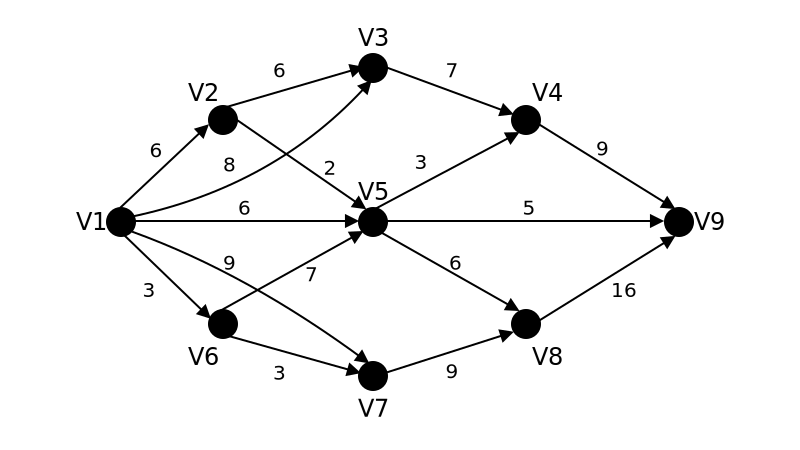
\includegraphics[width=360px]{7_flow}
\end{figure}
\begin{enumerate}
    \item Построение полного потока:
    \begin{align*}
        v_1 \rightarrow v_2 \rightarrow v_3 \rightarrow v_4 \rightarrow v_5\\
        \min\{6, 6, 7, 9\} = 6
    \end{align*}
    \begin{align*}
        v_1 \rightarrow v_8 \rightarrow v_7 \rightarrow v_6 \rightarrow v_5 \\
        \min\{3, 3, 9, 16\} = 3 
    \end{align*}
    \begin{align*}
        v_1 \rightarrow v_9 \rightarrow v_5\\
        \min\{6, 5\} = 5 
    \end{align*}
    \begin{align*}
        v_1 \rightarrow v_3 \rightarrow v_4 \rightarrow v_5\\
        \min\{8, 7-6, 9-6\} = 1
    \end{align*}
    \begin{align*}
        v_1 \rightarrow v_7 \rightarrow v_6 \rightarrow v_5\\
        \min\{9, 9-3, 16-3\} = 6
    \end{align*}
    \begin{align*}
        v_1 \rightarrow v_9 \rightarrow v_4 \rightarrow v_5\\
        \min\{6-5, 3, 9-7\} = 1
    \end{align*}
    $$ \Phi _{полн.} = 1 +6 +1 + 3+6 + 5 = 22$$
    \item Построение максимального потока:
    \begin{enumerate}
        \item $ v_1 \rightarrow v_3 \rightarrow v_2 \rightarrow v_9 \rightarrow v_4 \rightarrow v_5 $
        $$ \Delta_1 = \min\{8-1, 6, 2, 2-1, 9-8\} = 1$$ 
        \item $ v_1 \rightarrow v_3 \rightarrow v_2 \rightarrow v_9 \rightarrow v_6 \rightarrow v_5 $
        $$ \Delta_2 = \min\{8-2, 5, 2-1, 4, 16-9\} = 1$$ 
        \item $ v_1 \rightarrow v_7 \rightarrow v_8 \rightarrow v_9 \rightarrow v_6 \rightarrow v_5 $
        $$ \Delta_3 = \min\{9-6, 3, 7, 6-1, 16-9\} = 3$$ 
    \end{enumerate}
    $$ \Phi_{макс.} = 9 + 5+13=27$$
\end{enumerate}
Величина $|f|$ равна $27$.
\end{document}